\pagestyle{plain}
\setcounter{page}{1}

\chapter{Introduction}

In this thesis, we exploring the possibility of speeding  up cluster analysis by parallelization and dependency between input data properties and different parallelization approaches.\\
The main motivations for choosing this topic was a great growth in demand for processing large data. These data are collected from many sources such as social networks, financial markets, medical observation, space exploration or other scientific data. Even if this data seem like different, they have something in common. The first thing is that they contain may useful informations for scientists, sociologist, medics but even for business analysts, brokers or for advertisement. The second thing is that they must be processed by computers because of data size and compute time intensity. \\

Problem is that the data grows much faster than compute performance of the most modern hardware so neither computers have enough processing power for processing this data if we use standard algorithms. For this purposes there are known technologies for processing or simplifying big data including cluster analysis, generic algorithms, machine learning or simulation.
Problem is that in modern big data world neither of these techniques in conjunction with traditional hardware are enough so we are enforced to use other possibilities. \\
Because processing single data is not so complex and processing them is very often independent, ideal hardware should contains many of simple and cheap compute units capable of operating in parallel on huge amount of data. This is exactly way followed by manufacturers of the most modern hardware, which is not designed for the highest performance of individual cores but for the best parallel work reached by increasing number of cores on single chips and speeding up communication between cores. \\

As a reasonable solution is to use compute performance of graphics cards which contains thousands of simple cores. Even though their purpose is primarily graphical tasks, cards allows to use theirs power to common computations (general-purpose computing on graphics processing units - GPGPU). Their performance with each generation increases rapidly so they are great opportunity for making current compute-intensive algorithmic problems efficient and less time-consuming and make them usable for areas in which their application was inefficient or even not possible.\\
Because graphical cards was originally specialized for computation of graphical primitives, which contains many of separate and independent tasks so the problem is when we need to process tasks which are not so similar to graphical primitives. This is usually the problem of processing big data in some more sophisticated way and we must solve the problem with dependencies between single computations. \\

As a representative of such problems we chose cluster analysis, especially k-means algorithm - algorithm, which is looking for clusters in the input data and finds a representative (called mean or centroid) of each cluster. It works iteratively and in each step, it finds nearest representative for each object and than compute new representative for each cluster. This algorithm has a very broad scope of application and it is very time consuming for big data so it is really useful to accelerate it using the most modern hardware.\\

Problem is that this algorithm contains several compute and data dependencies which must be solved. We could easily compute the nearest representative for each object but problem is when we want to compute update representative from object assigned to same cluster. Because we have large number of objects and so large number of compute cores, we want to parallelize the computation in object manner - each object is processed by single core. Problem is that we need to accumulate data for each of the newest representative and problem is, that it could be accessed by many cores at a time. We must choose some synchronization primitive, which slows down the computation, or choose a different way of parallelizing this task such as parallelizing computation in representative manner - each new representative is processed by single compute core and it iterates through all objects which could be slow too.\\

There are also problems with data size and memory usage efficiency. GPU has several types of memory. They differ significantly in size and latency - bigger memory is usually slower with bigger latency and vice versa, smaller memory is faster with small latency times. The main goal is to use the memory as effectively as possible. Problem is that the big input data are sometimes much larger than the biggest GPU memory so we must design a way, how to swap data between host and GPU and between GPU's memory effectively. This is problem because of variety of input data so we must try several versions and find out which approach is the best with respect to the different input data.\\

We must solve this by modification of the k-means algorithm to GPU environment and develop several versions to find out which approach fits the best for concrete type of data.

\chapter{Cluster Analysis} \label{sec:clusteranalysis}
Cluster analysis is a task that groups objects from the input set so that each group consists of objects with similar properties. Similar means that same property of two objects differs minimally in comparsion to same property of other objects. This means that each cluster contains objects that are more similar than objects from other groups. Hence the cluster analysis may be performed only on sets of objects of which must each be described by the same set of properties. This analysis has a wide range of applications, such as data mining, pattern recognition, machine learning, and many more.\\
Cluster analysis itself is only a task to be solved, not a concrete algorithm. There are many ways to solve this task, but they differ significantly in defining what cluster is and in cluster search efficiency. Most commonly definitions of the cluster are groups with small distances between the objects from the same cluster, dense areas of the input data, intervals or each particular statistical distribution.\\
As a distance we take a function $d:M\times M \to \mathbb{R}$ fulfilling following rules:\\ \\
$ \forall  a,b,c \in M$
\begin{enumerate}
\item $d(a,b)\geq 0$ \textit{(non-negativity)}
\item $d(a,b) = 0 \iff a = b$ \textit{(identity)}
\item $d(a,b) = d(b,a)$ \textit{(symmetry)}
\item$d(a,b) \leq d(a,c) + d(c,b)$ \textit{(triangle inequality)}
\end{enumerate}
There are also two types of cluster organization. One way is hierarchically ordered clusters creates which creates a system of subsets where the intersection of the two is either the empty set or just one of them or non-hierarchical clusters, which creates system where clusters are disjoint sets. Because of complexity of the hierarchical clustering, in this thesis we deal with non-hierarchical type only.

\section{Cluster Models and Algorithms} \label{sec:clustermodels}
There are so many cluster models and one of the reasons why there exists a large amount of them is that the ``cluster'' cannot be precisely defined~\cite{EstivillCastro02}. Second reason is really wide applicability of this task so people from different departments approach this problem differently, because their notion of cluster differs significantly. \\

There exist many clustering algorithms because of many cluster models but there exist no universal algorithm, such an algorithm that covers all cluster models. Each algorithm was designed to cover one model or a subset of models and usually it is weak or not applicable for other models.\\
Because all of these algorithms counts distance, appropriate metric must be used. Some commonly used metric are:
\begin{description}
\item[Manhattan distance $L_1$] $$\|a-b\|_1=\sum_i |a_i - b_i| $$
\item[Euclidian distance $L_2$] $$\|a-b\|_2=\sqrt{\sum_i (a_i - b_i)^2 }$$
\item[Squared Euclidian distance $L_2^2$] $$\|a-b\|_2^2=\sum_i (a_i - b_i)^2 $$
\item[$p$-norm distance $L_p$] $$\|a-b\|_p=\Big(\sum_i |a_i - b_i|^p\Big)^\frac{1}{p} $$
\item[Maximum distance $L_\infty$] $$\|a-b\|_\infty=\lim_{p\to\infty}\Big(\sum_i |a_i - b_i|^p\Big)^\frac{1}{p}=\max_i |a_i - b_i| $$
\end{description}
All of these methods are only applicable for numeric data, so for other types, different metrics must be used (for example, Levenshtein for text, Mahalanobis for distance between point and distribution).
\\
The most typical models of clusters and algorithms are:
\begin{description}
\item[Well-Separated Clusters] Objects are well separated. Cluster is a set of objects such that each object in cluster is closer to objects from its cluster than to objects from other clusters~\autoref{fig:wellSeparatedObjects}. This is the easiest data input and most of algorithms performs well in this case.

\item[Center-Based Clusters] Object belongs to cluster if it is closer to the ``center'' of the cluster than ``centers'' of all other clusters.~\autoref{fig:centerBasedClusters} Center of cluster is usually called centroid or mean and it could represents whole cluster. This is good model for k-means like algorithms. \\
\textit{\textbf{Center-based clustering}} representing clusters as central object, which may not be part of the input data set.  For example \textit{\textbf{k-means}} algorithm takes $k$ centers and than each object is assigned to nearest center. Again, many metrics could be used, but commonly \textit{Euclidian distance} or \textit{Squared Euclidian distance} is used. \textit{\textbf{k-means}} clustering is basically an optimization problem where we looking for $k$ centers so distances will be the lowest possible. Problem is that optimization itself is NP-hard problem, so solution is commonly only approximate solution is searched. Approximation is commonly done by many iterations consist of assigning clusters to objects and  counting new means.
There are many variants of \textit{\textbf{k-means}} algorithm, they will be described later %TODO add ref too kmeans section
%\begin{description}
%\item[k-medoids] - centers are only objects from input data set
%\item[k-medians] - median is used instead of mean
%\item[k-means++] - initial centers are chosen randomly
%\item[Fuzzy k-means] - fuzzy cluster assignment is allowed
%\end{description}

One of the biggest problems of \textbf{k-means} algorithms is that the number of clusters must be specified at the beginning. Second problem is that clusters with similar size are used (in term of distance, not number of contained objects). This usually leads to splitting bigger clusters into smaller ones, because algorithm optimize cluster centers, not borders.
Output of \textit{\textbf{k-means}} like algorithms is usually input data set split in \textit{Voronoi cells}which could be useful for some problems.

\item[Contiguous Clusters] This model is similar to Center-Based Clusters model but there is difference that two clusters can merge into one. In other words, object is in cluster if it is similar to one ore more other objects from cluster.~\autoref{fig:contiguousClusters}\\
Main idea of \textbf{Contiguity-based clustering} is that objects that are nearby are more related than objects that are farther, so these algorithms grouping objects based on their distance only. Each cluster can be described by sum of distances or by maximum distance needed to connect objects in cluster. Having these cluster property, they can be easily ordered into hierarchy so parent clusters needs little more distance to connect its objects. This hierarchy could be represented as a dendrogram, which is tree diagram showing cluster hierarchy.\\

Other problem is the selection of linkage criterion, because cluster consists of many objects, there are many choices to compute the distance to. There are several methods for choosing linkage criteria between two sets of objects $A$ and $B$, $d$ is chosen metric:
\begin{description}
\item[Maximum or complete linkage clustering] $$\max\{d(a,b) : a \in A, b \in B\}$$
\item[Minimum or single linkage clustering] $$\min\{d(a,b) : a \in A, b \in B\}$$
\item[Mean or average linkage clustering, or UPGMA] (Unweighted Pair Group Method with Arithmetic Mean) $$\frac{1}{|A||B|}\sum_{a \in A} \sum_{b \in B} d(a,b)$$
\item[Centroid linkage clustering, or UPGMC] (Unweighted Pair-Group Method using Centroids) $$\|c_a - c_b\| \mbox{ where } c_a \mbox{ and } c_b \mbox{ are the centroids of clusters } A \mbox{ and } B$$
\item[Minimum energy clustering] $$\frac{2}{nm}\sum_{i,j=1}^{n,m}\|a_i-b_j\|_2-\frac{1}{n^2}\sum_{i,j=1}^{n}\|a_i-a_j\|_2-\frac{1}{m^2}\sum_{i,j=1}^{m}\|b_{i}-b_{j}\|_{2}$$
\end{description}

These methods are not resistive for extreme objects, which cause generating new clusters or even merging others. Methods has generally $O(n^3)$ complexity so they are slow for large amount of data. There exist optimization for special cases which has only complexity $O(n^2)$. These methods are taken as obsolete.

\item[Density-Based Clusters] Clusters are dense regions of objects. They are separated by low-density regions. This method is useful when some noise is present because the low-density regions will cover them and clusters will not change.~\autoref{fig:densityClusters} \\
Clusters in \textbf{Density-based clustering} are defined as areas with higher density of objects than in the rest of input data. Standalone objects are taken as noise. One of the most popular method is \textit{DBSCAN}. It is similar to contiguity-based clustering, because it connecting points based on the distance, but it only connects points satisfying density criterion. This means that in neighborhood specified by distance must be a minimum number of objects. These objects are called core objects and form the basis of cluster. Than objects which do not satisfy the density criterion but are close enough to at least one point from the cluster are added to cluster too.\\
The advantage of this method is its computational modesty, because it require only linear number of range queries. This method is deterministic so there is no need to tun it in iterations.
Drawback of these methods is the $\epsilon$ density parameter so borders of clusters with smaller density could be interpreted as  noise. Also separating nearby clusters may cause problems to these methods.

\item[Distribution models] Clusters in distribution models are objects that belong to same probability distribution. It is possible that one object belongs to more clusters.\\
In \textbf{Distribution-based clustering}, clusters are defined as objects from the same or similar distribution. This approach basically emulates process of generating the input data and try to reconstruct the lost statistical parameters. Main problem of this typ of clustering is problem known as \textit{overfitting}. This means that more complex model is described by less complex one and the difference between them is marked as deviation or noise. For example 3 points from the neighborhood of parabola vertex will be described by linear function.\\
One of methods used in distribution-based clustering is \textit{Gaussian mixture models} where algorithm iteratively optimizing parameters of fixed number of Gaussian distributions.
Problem is that this method assuming Gaussian distributed data set, but this set may not have even a model.

\item[Conceptual Clusters] Objects in cluster has some properties same or similar, but other properties could differ significantly.~\autoref{fig:conceptualClusters}\\
As algorithm for Conceptual Clusters, we can use algorithm depends on other model properties and less significant properties of objects could be easily omitted.

\item[Graph-Based Models] For example cliques in graphs should represent clusters. Clique is subset of nodes where every two nodes are connected with edge.~\autoref{fig:graphClusters}\\
Because of special demands of this model, special algorithms are needed so we could use graph algorithms, for example Bron-Kerbosch algorithm for finding cliques. %TODO source!
\end{description}

\begin{figure}[h]
\centering
\begin{subfigure}{.49\textwidth}
  \centering
  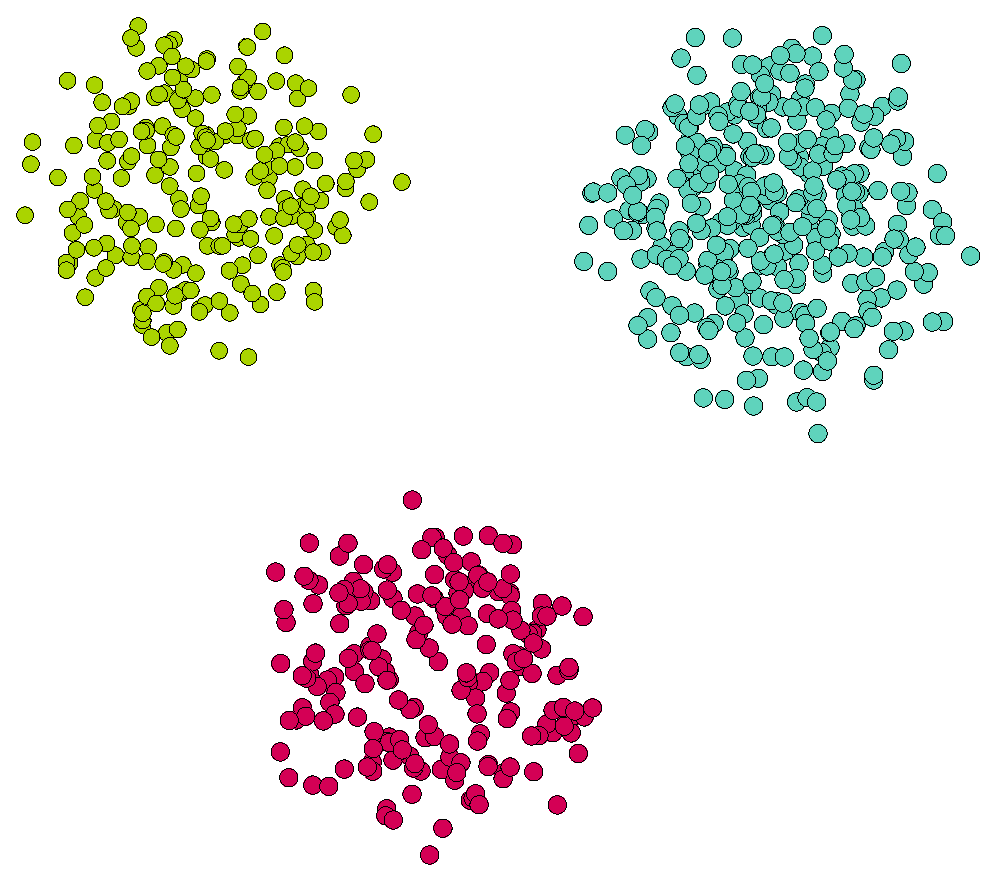
\includegraphics[width=.5\linewidth]{img/wellSeparatedObjects.eps}
  \caption{Well sepatated objects}
  \label{fig:wellSeparatedObjects}
\end{subfigure}
\begin{subfigure}{.49\textwidth}
  \centering
  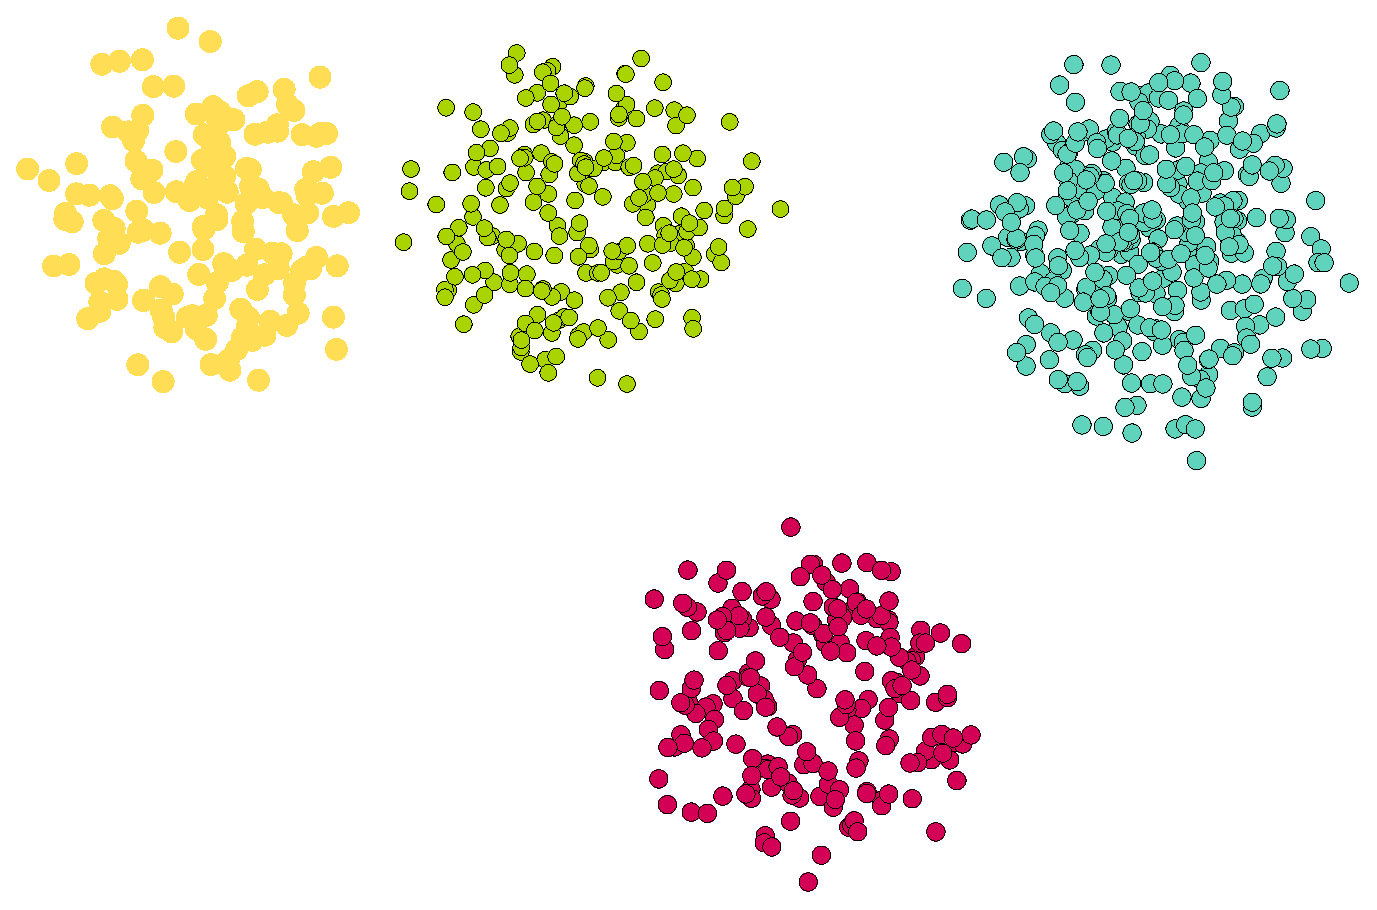
\includegraphics[width=.5\linewidth]{img/centerBasedClusters.eps}
  \caption{Center-Based Clusters}
  \label{fig:centerBasedClusters}
\end{subfigure}
\vspace*{0.5cm} 
\begin{subfigure}{.49\textwidth}
  \centering
  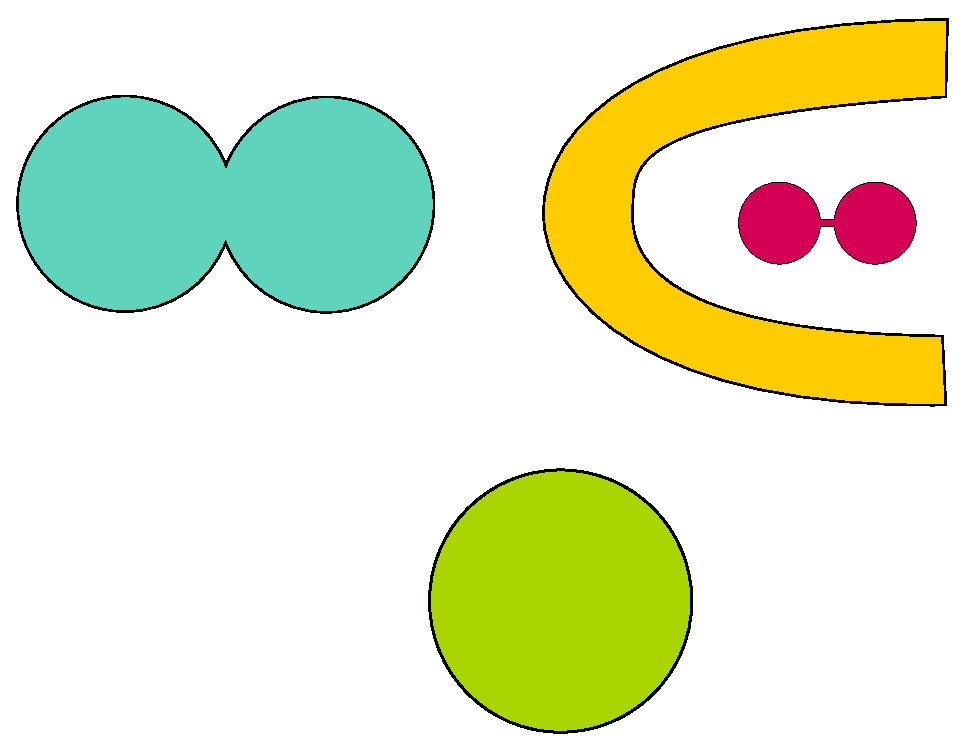
\includegraphics[width=.5\linewidth]{img/contiguousClusters.eps}
  \caption{Contiguous Clusters}
  \label{fig:contiguousClusters}
\end{subfigure}
\begin{subfigure}{.49\textwidth}
  \centering
  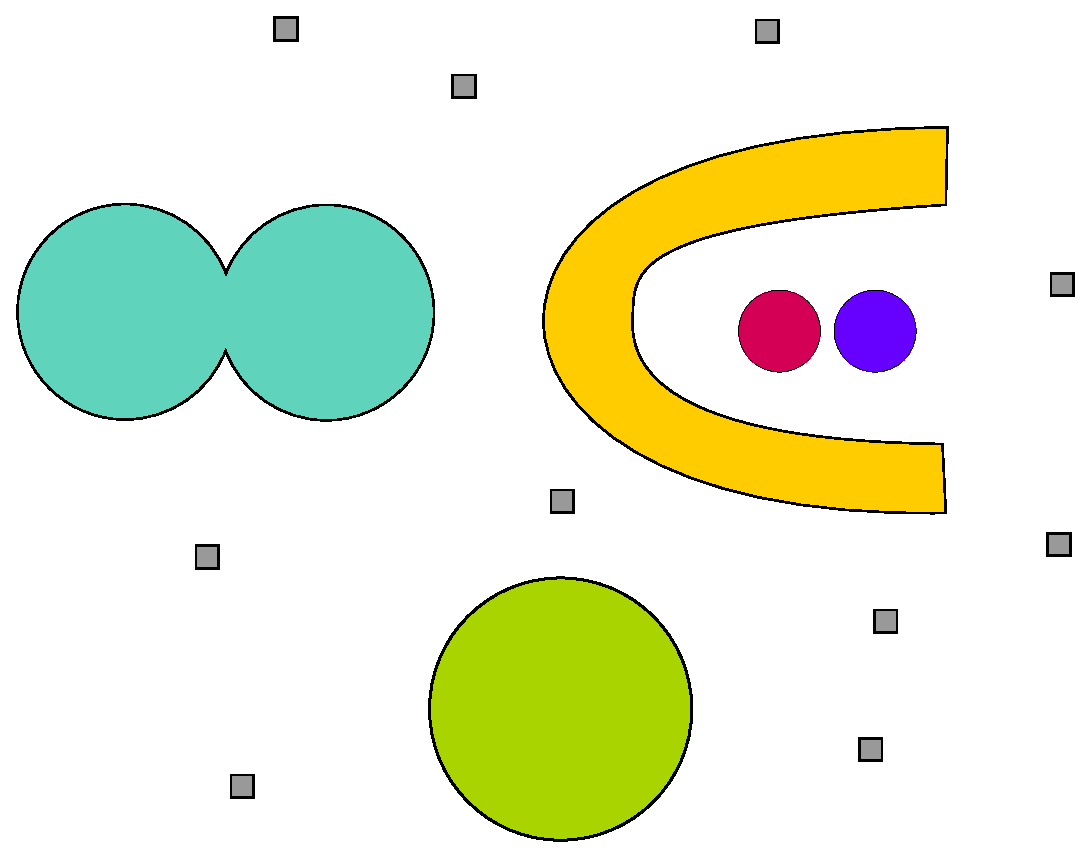
\includegraphics[width=.5\linewidth]{img/densityClusters.eps}
  \caption{Density-Based Clusters (Gray squares represent noise)}
  \label{fig:densityClusters}
\end{subfigure}
\vspace*{0.5cm} 
\begin{subfigure}{.49\textwidth}
  \centering
  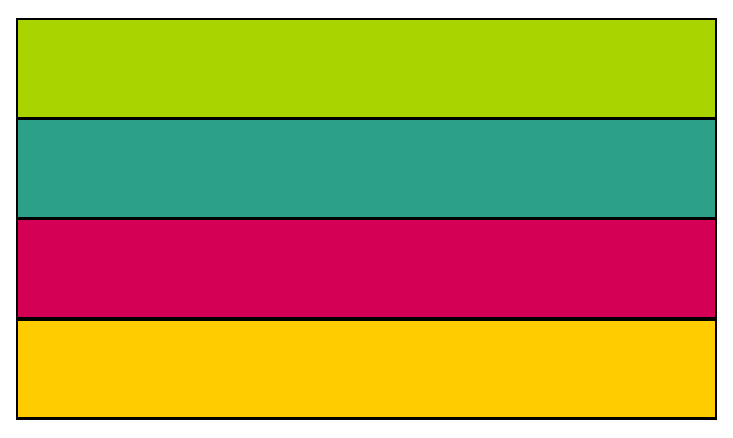
\includegraphics[width=.5\linewidth]{img/conceptualClusters.eps}
  \caption{Conceptual Clusters (Points in cluster have y-coordinate from specific range, omitting x-coordinate)}
  \label{fig:conceptualClusters}
\end{subfigure}
\begin{subfigure}{.49\textwidth}
  \centering
  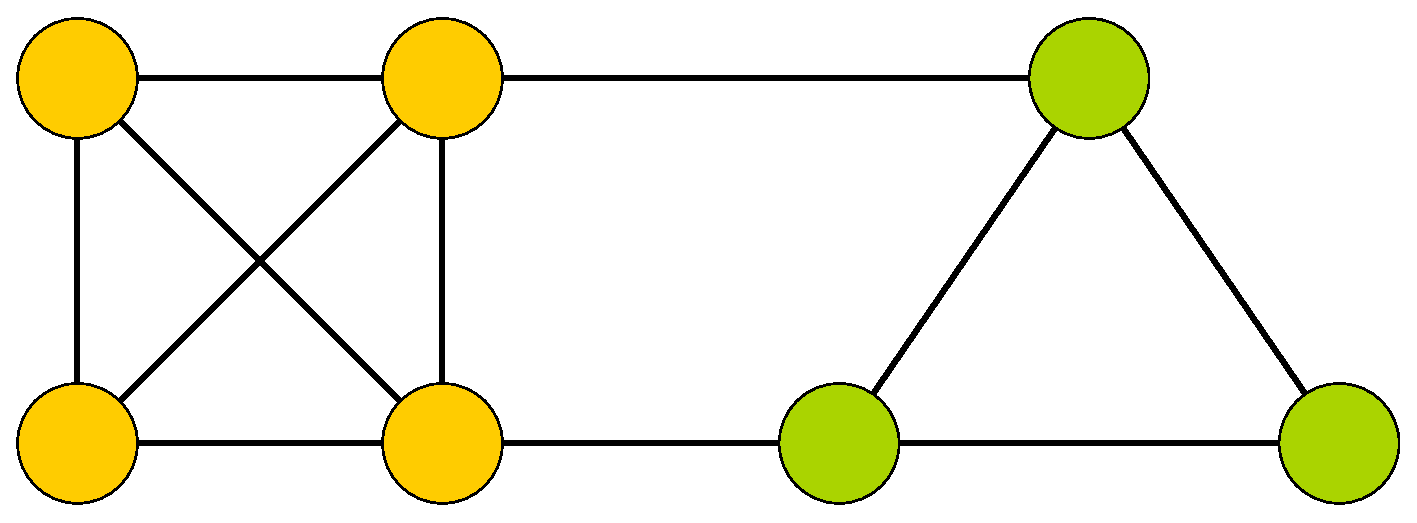
\includegraphics[width=.5\linewidth]{img/graphClusters.eps}
  \caption{Graph-Based Clusters}
  \label{fig:graphClusters}
\end{subfigure}
\caption{Typical cluster models}
\end{figure}

\vspace{8 mm}
\noindent
There is also another option for splitting clustering algorithms by type of objects relationship: 

\begin{description}
\item[Strict partitioning clustering] Objects belongs exactly into one cluster
\item[Strict partitioning clustering with outliers] Same as \textit{\textbf{strict partitioning clustering}} but isolated objects can be also unassigned. 
\item[Overlapping clustering] Object may belong to multiple clusters and we can specify, how much object belong to each cluster for example in percent.
\item[Hierarchical clustering] Object belongs also into parent clusters.
\end{description}
 \pagebreak
\chapter{General-Purpose Computing on Graphics Processing Units}
General-Purpose computing on graphics processing unit (GPGPU) is the use of graphics processing unit (GPU) and central processing unit (CPU) together for acceleration data-intensive or compute-intensive tasks. Main advantage of GPUs is that in comparison with ordinary CPU, they have ten times, a hundred times but sometimes thousand times more cores, so if the task is parallelizable, it could be accelerated up to thousand times on GPU in comparison to serial CPU version. At the beginning, GPUs support only computation of vectors or matrices, usually two, three or four dimensional for graphical purposes, so general purpose computation had to be reformulated to this graphical principles supported by major graphics APIs like DirectX or OpenGL. Later, Nvidia CUDA and OpenCL frameworks solve this problem and allows to programmer to ignore graphics environment. Main difference between this two frameworks is that CUDA is only for Nvidia graphics cards so it could use concrete hardware specific properties. OpenCL is a universal vendor independent framework for parallel computations and can be run on wide range of devices like GPUs and CPUs, but , but it is not so good for high performance computing as CUDA because of wide range of covered devices so it could not use architecture and hardware specific properties.
\subsection{GPU and CPU comparison} \label{ssec:gpucpucomparison}
Main difference between CPU and GPU is in their specialization. Instead of general purpose of CPUs, GPUs are specialized on graphics, which is easily parallelizable, so GPU architecture is targeted for parallel work. After GPGPU was introduced, problem with GPU specialization was solved and GPUs began to compete with processors. Main differences between CPUs and GPUs are:
\begin{description}
\item[Number of cores] CPU has only few physical cores~\autoref{fig:cpuarchitecture}, sometimes virtually doubled. Common home CPUs have a maximum around 8 logical cores, server CPUs could have more, but maximally slightly less than a hundred cores. Compared two that, modern GPUs have around five hundred cores~\autoref{fig:gpuarchitecture}, the best models have around five thousand cores, so they have great potential for parallel tasks.
\item[Core architecture] GPU cores are specialized for numeric computations, not for general tasks as CPU cores, but because of their specialization, they compute numeric tasks really fast. \item[Threads] Approach to threads is different. CPU can process threads from different tasks at one time, which is called Simultaneous Multithreading (SMT), GPU uses Simple Instruction Multiple Thread (SIMT) pattern, which means that multiple threads run on same code and based on their identification, they could work on different branches or access different data.
\item[Memory] CPUs use big cache memory for hide latency of memory access so when thread is switched to different core, there is problem witch locally cached data, which are useless on original core and must be re-cached on new core. GPU has only small caches, because most of memory is on device, so context switch can be performed really fast.

\begin{figure}[h]
\centering
\begin{subfigure}{.5\textwidth}
  \centering
  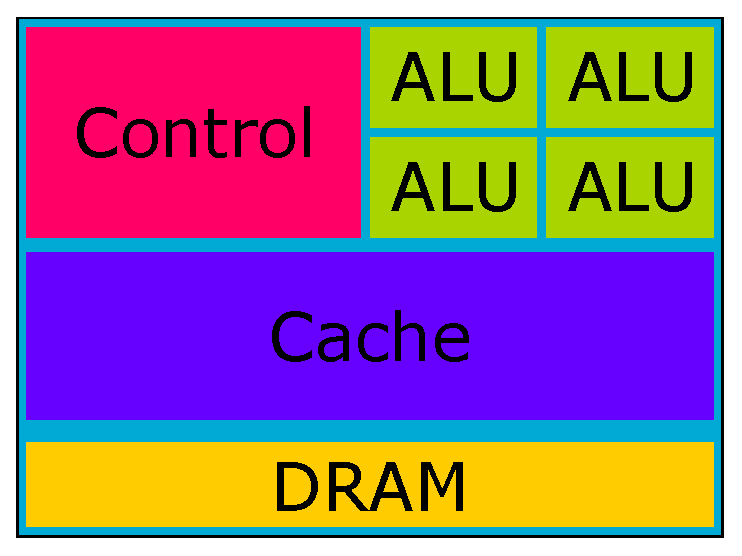
\includegraphics[width=.8\linewidth]{img/CPUarchitecture.eps}
  \caption{CPU architecture}
  \label{fig:cpuarchitecture}
\end{subfigure}
\begin{subfigure}{.5\textwidth}
  \centering
  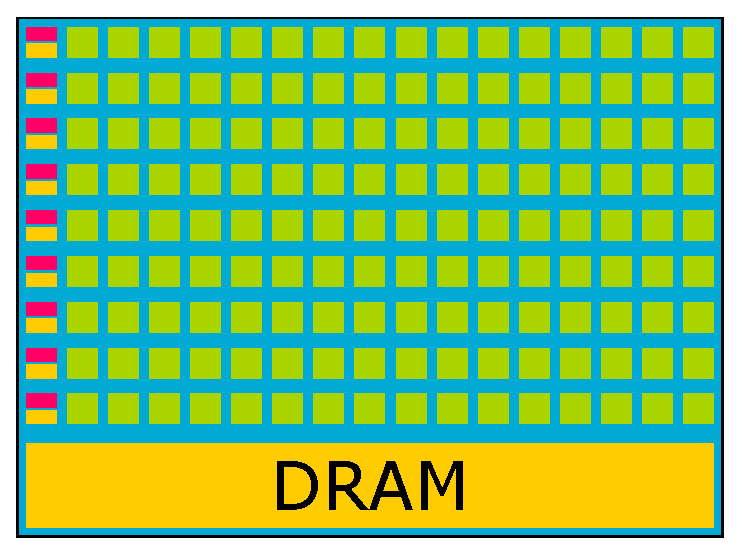
\includegraphics[width=.8\linewidth]{img/GPUarchitecture.eps}
  \caption{GPU architecture (Fermi)}
  \label{fig:gpuarchitecture}
\end{subfigure}
\caption{CPU and GPU architecture comparison}
\end{figure}

\end{description}
%\begin{table}
%\begin{tabular}{|l|l|l|}
%\cline{1-2}
%NIC & CPU & GPU \\ \cline{1-2}
%# cores & Few cores per chip & Many cores per chip \\ \cline{1-2}
%Specialization & General purpose cores & Cores psecialized for numeric computations \\ \cline{1-2}
%Threads approach & Processing different threads & SIMT thread processing \\ \cline{1-2}
%Memory access & Huge caches to reduce memory latency & Huge amount of threads and fast context switch \\ \cline{1-2}
%\end{tabular}
%\end{table}
\subsection{Compute Unified Device Architecture (CUDA)}
CUDA is parallel computing platform developed by Nvidia. This includes hardware and software architecture integrated on Nvidia graphics cards. There exist more solutions than this one from Nvidia, but CUDA is one of the best for high performance computing. The main advantage over OpenCL and other solutions is a direct link to the hardware, which is not the case of OpenCL, because it supports a large range of hardware divergent devices so it can't use concrete hardware advantages. \\
Nvidia use Simple Instruction Multiple Thread (SIMT) model, which is more flexible than Simple Instruction Multiple Data (SIMD), but generally, it has less performance. Both models approaching parallelism by by broadcasting same instruction to multiple execution units, so only one instruction fetch/decode unit is needed by many execution units. Difference is that SIMT also have multiple register sets and addresses. Main difference is that SIMD processes short vectors in parallel and always all threads do the same work. For example, when we need sum two vectors, SIMD must iterate through vectors and in one step, it can only process as many elements as a computing units count is. On CUDA with SIMT model, we launch as many threads as size of vector and each thread can store values in own register. Not all threads run actually in parallel, but many of them do.\\
CUDA architecture contains larger processors called \textbf{Symmetric Multiprocessor (SM)}. The oldest is \textbf{SMP} - Fermi~\autoref{fig:smparchitecture}, \textbf{SMX} - Kepler~\autoref{fig:smxarchitecture} and the newest \textbf{SMM} - Maxwell~\autoref{fig:smmarchitecture}. Each SMP contains processor cores with registers (from 32 on Fermi architecture, 128 on Maxwell architecture and 192 on Kepler architecture), load/store units (LD/ST), Special Function Units (SFUs), shared instruction cache, shared memory and data caches. LD/ST and SFUs are shared by groups of cores, size of group depends on architecture.\\
Versions of CUDA are referred as \textbf{Compute Capability} (CC). This CC describe the device characteristics and a set of instructions that are supported. CC is tightly coupled with architecture (CC 1.x was supported by Tesla architecture, CC 2.x by Fermi, 3.x by Kepler, 5.x by Maxwell).

\subsubsection{Execution model}

\begin{figure}[h]
  \centering
  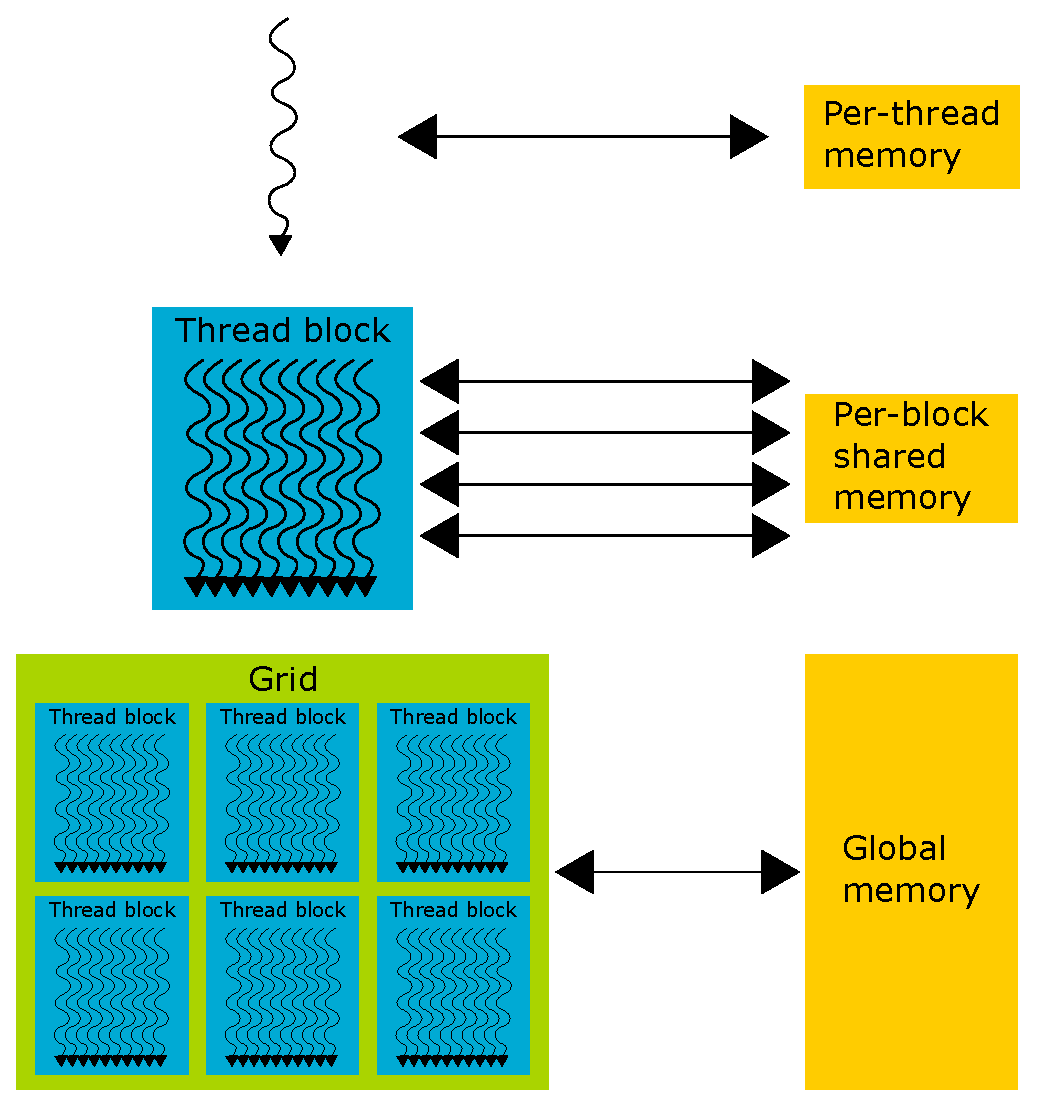
\includegraphics[width=0.8\linewidth]{img/CUDAExecutionModel.eps}
  \caption{CUDA Execution model}
  \label{fig:cudaexecmodel}
\end{figure}

Parallel programming on CUDA architecture contains two layers of parallelization~\autoref{fig:cudaexecmodel}. The first layer of parallelization is called \textbf{Grid} and it is handled by single GPU chip. Grid consists of blocks which are mapped to Symmetric Multiprocessors, each SM handle one or more \textbf{blocks} but block is never handled by more than one SM. The second layer (Block) consist of \textbf{threads} which runs on cores. The block size could be even bigger than number of cores on SM, than only part of block is run simultaneously. This part is called \textbf{Warp}.\\ Maximum number of currently running blocks and threads in each block depends on architecture, because each architecture has different number of SMs and SM has different number of compute cores. Threads in one block could be executed concurrently or serially and no particular order, but it can be coordinated by synchronizing threads.\\

\begin{figure}[p]
\centering
\begin{subfigure}{0.49\textwidth}
  \centering
  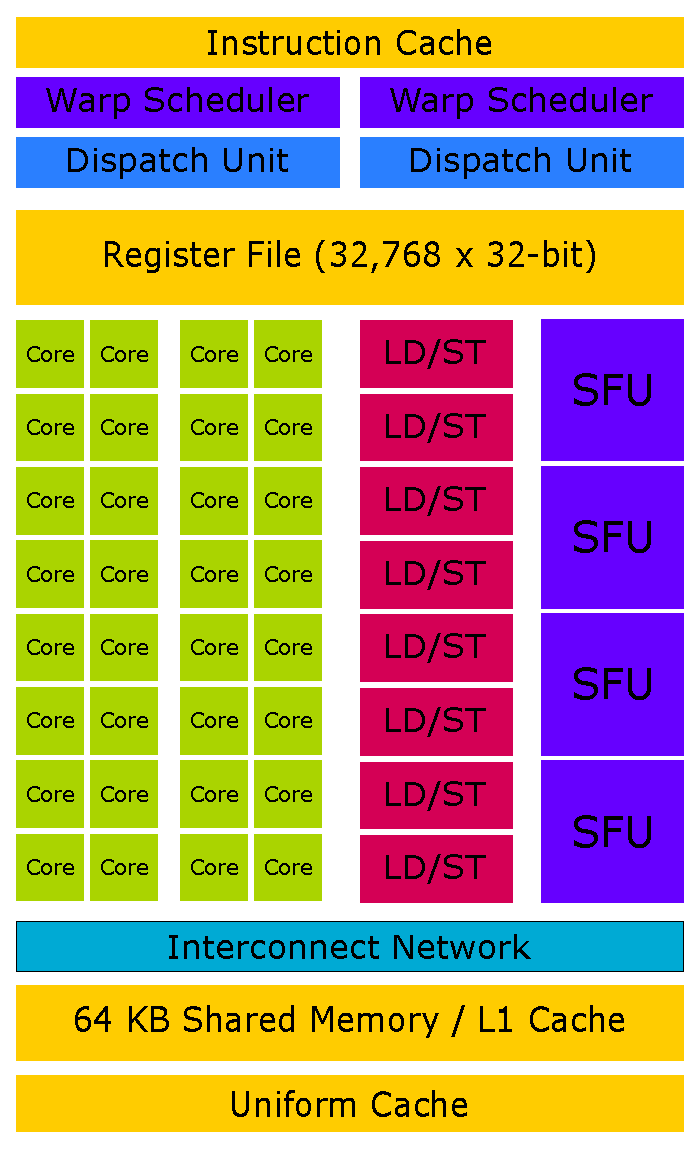
\includegraphics[width=0.8\linewidth]{img/SMPArchitecture.eps}
  \caption{SMP architecture}
  \label{fig:smparchitecture}
\end{subfigure}
\begin{subfigure}{0.49\textwidth}
  \centering
  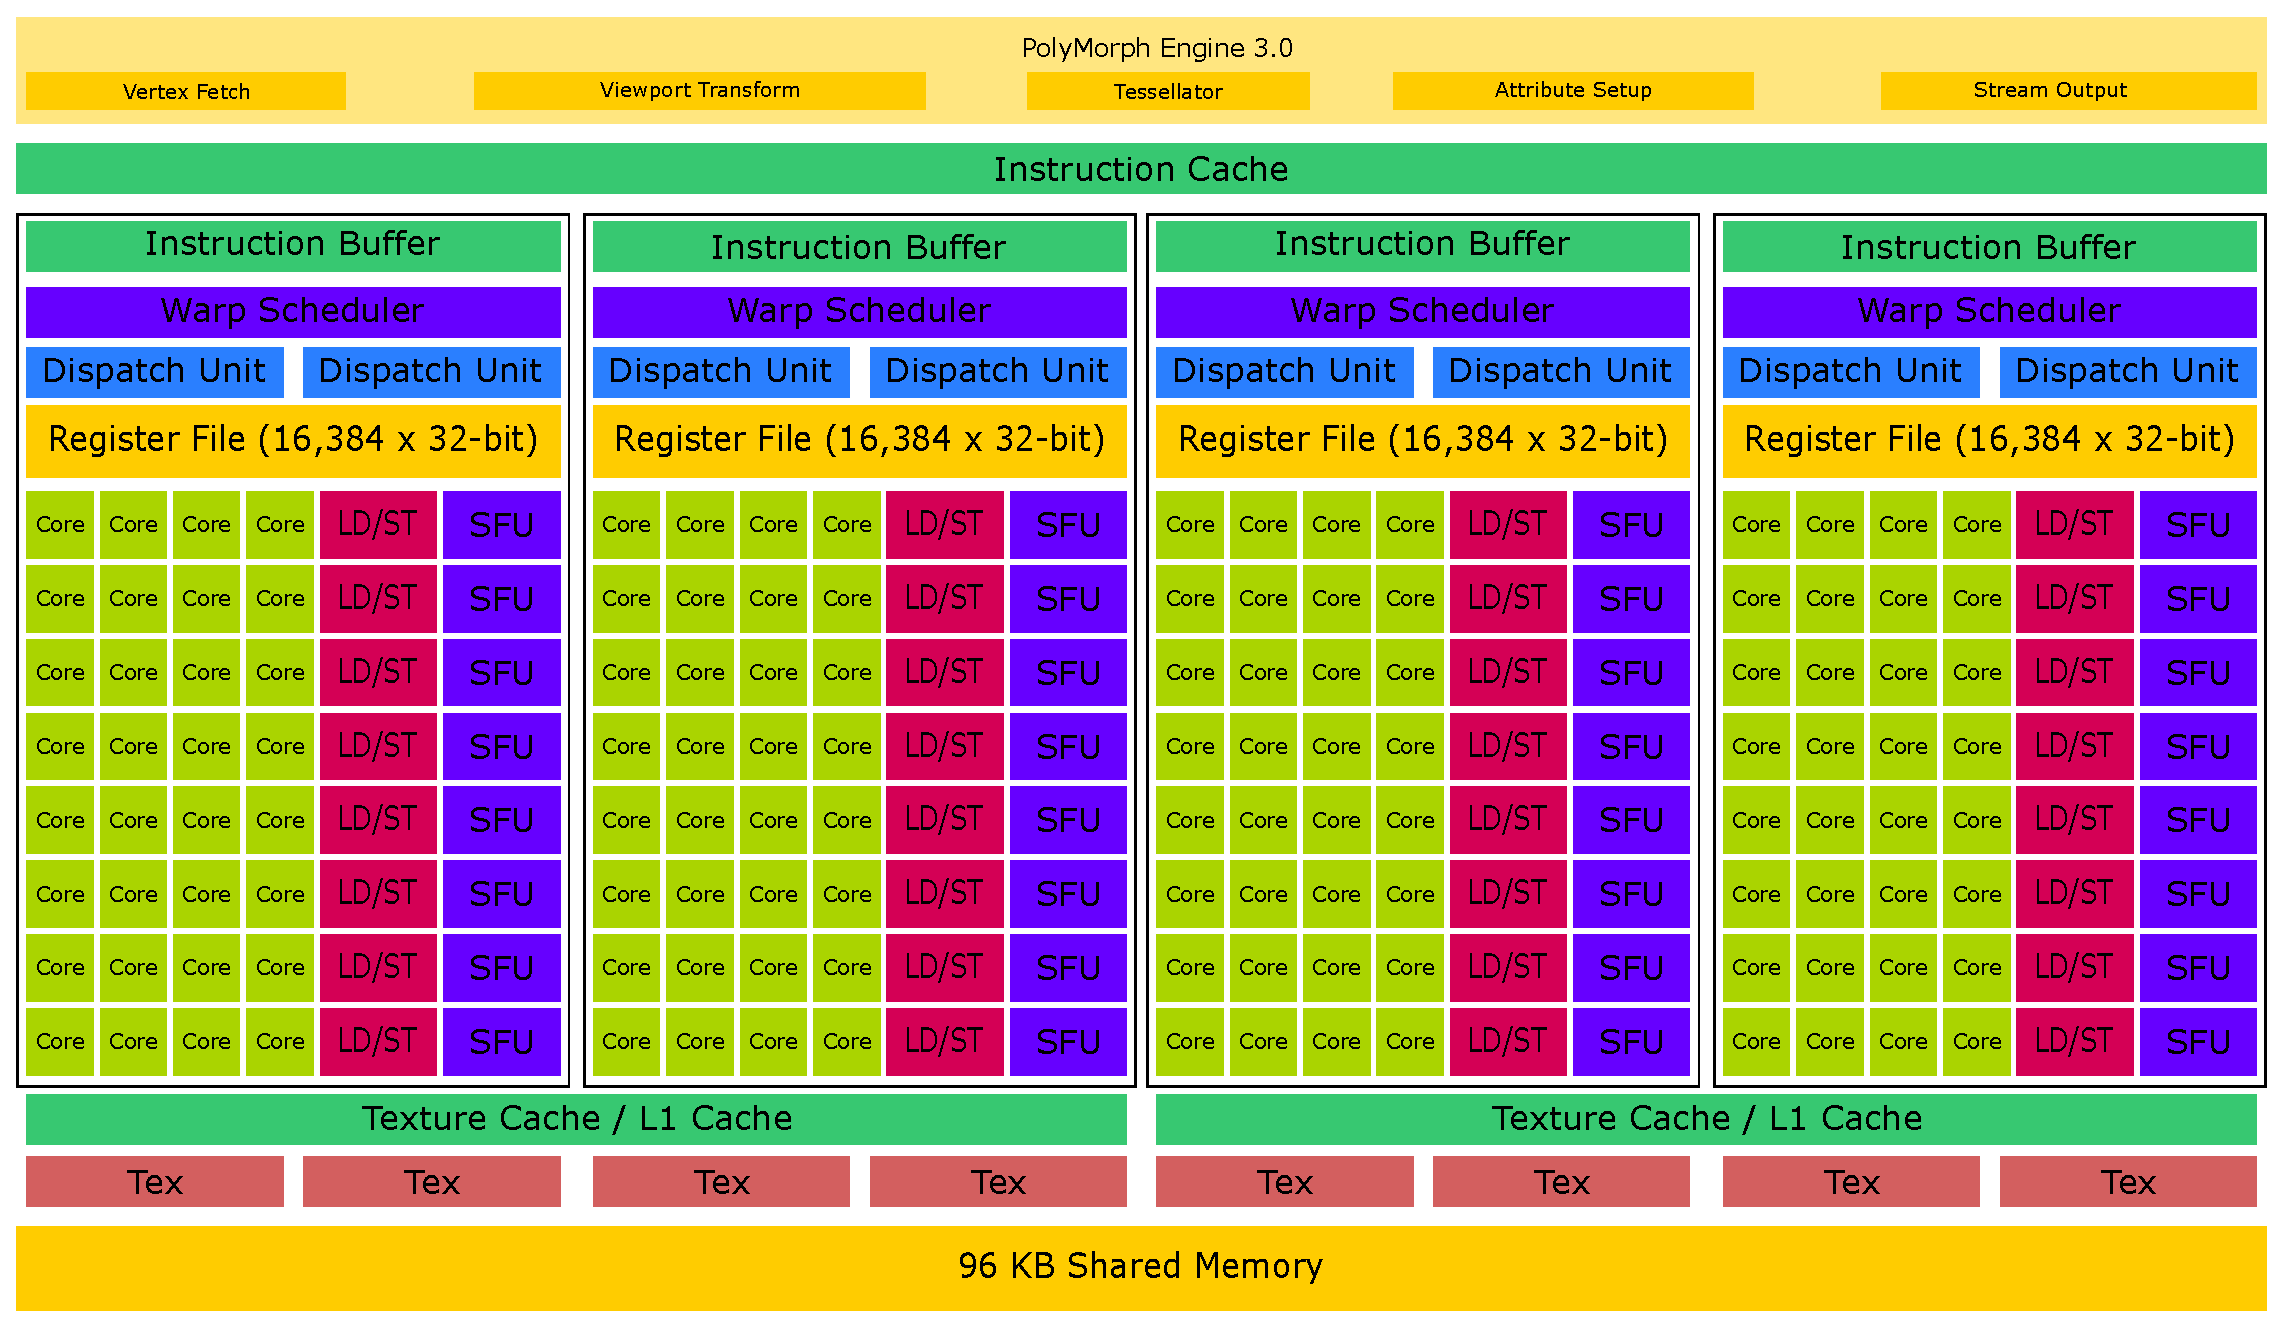
\includegraphics[width=1\linewidth]{img/SMMArchitecture.eps}
  \caption{SMM architecture (Fermi)}
  \label{fig:smmarchitecture}
\end{subfigure}
\vspace*{0.1cm} 
\begin{subfigure}{0.6\textwidth}
  \centering
  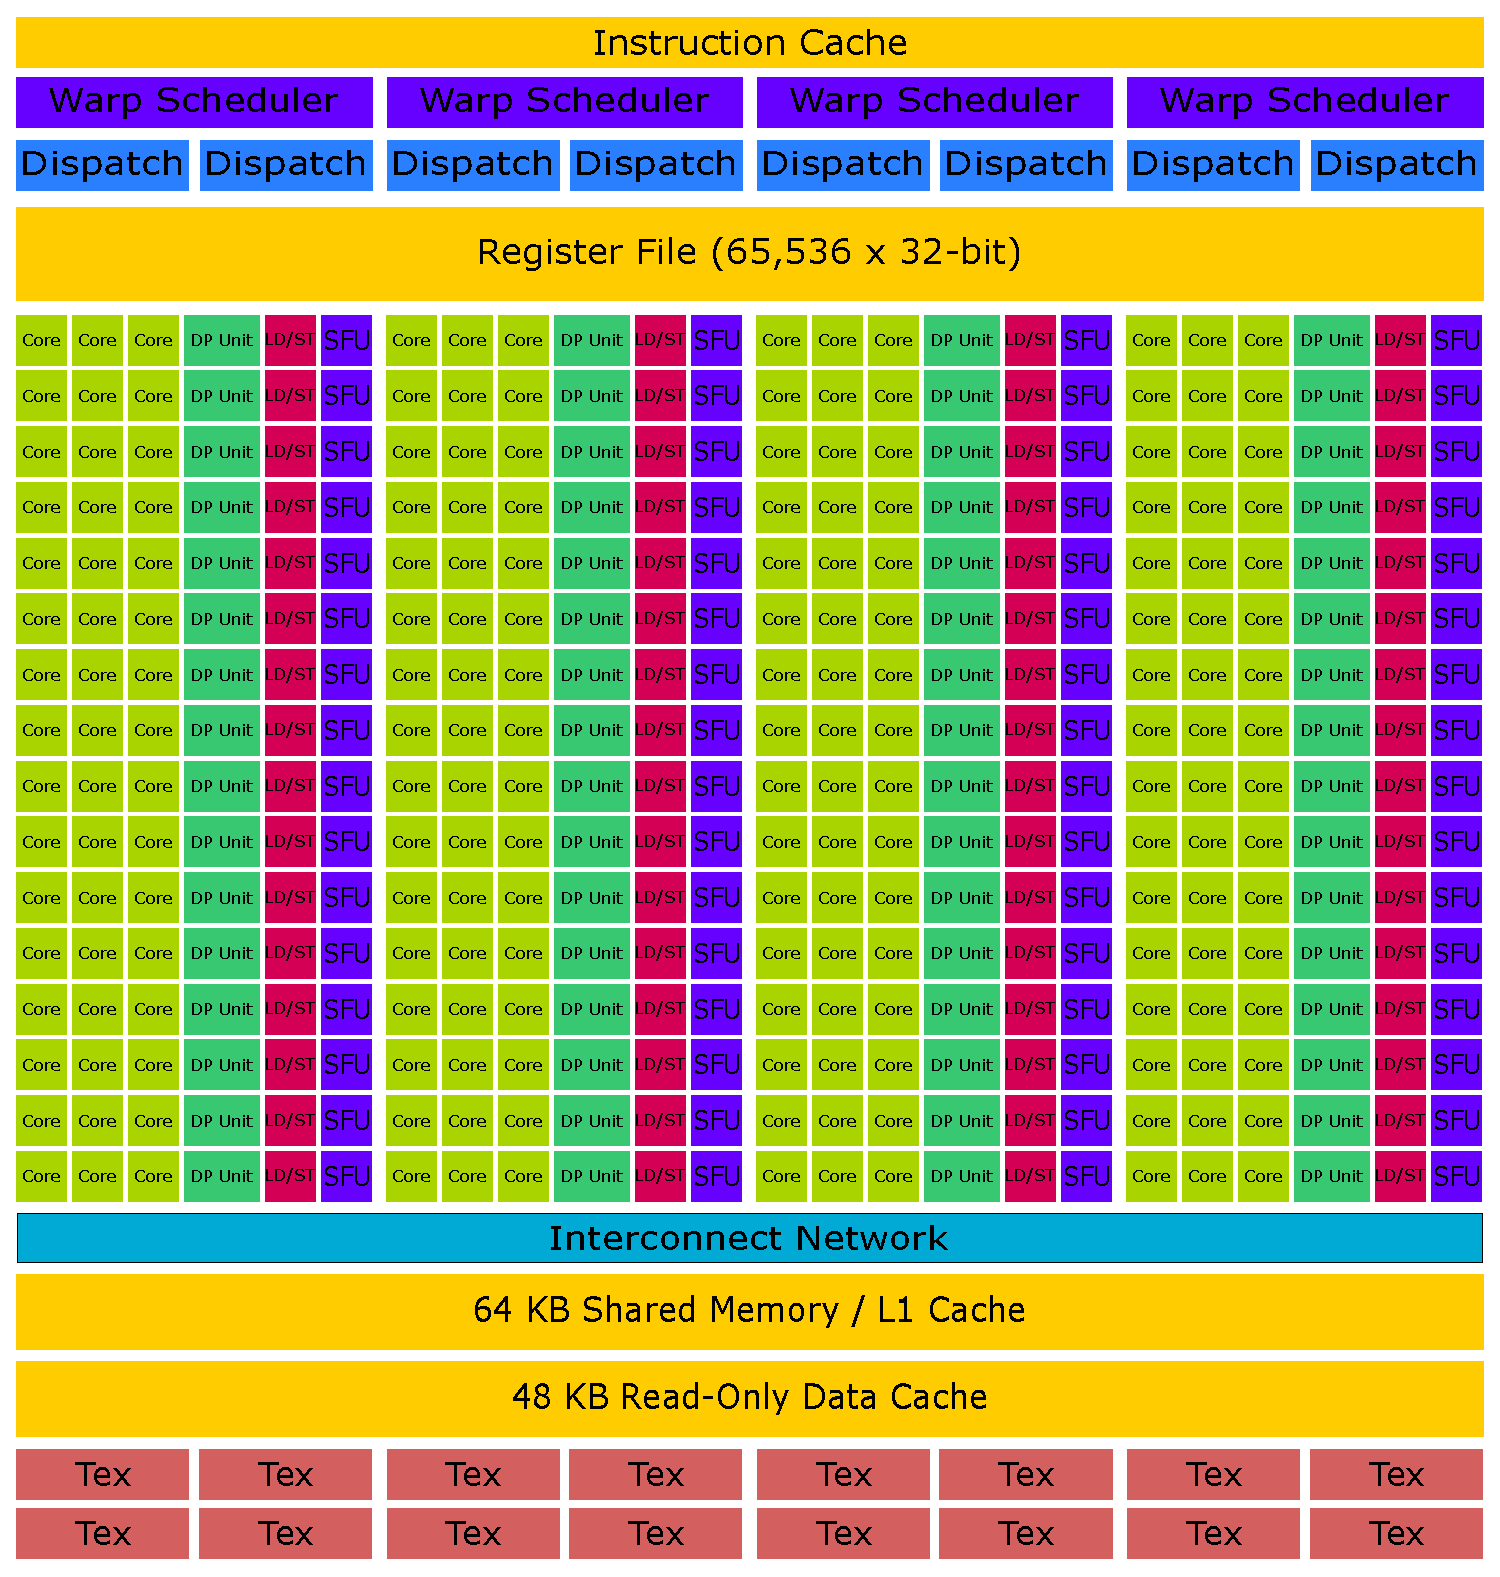
\includegraphics[width=0.9\linewidth]{img/SMXArchitecture.eps}
  \caption{SMX architecture (Fermi)}
  \label{fig:smxarchitecture}
\end{subfigure}
\caption{CPU and GPU architecture comparison}
\end{figure}

\subsubsection{Memory model}

Memory model on CUDA architecture~\autoref{fig:cudamemaccess} contains more types of memory which differs mainly in size, bandwidth and latency.
\begin{description}
\item[Global memory] is off the chip, but on the device. It is the largest memory (GBs) and it has high bandwidth (~100 GBps) but high latency (400-600 clock cycles). It is operated in transactions of 32B - 128B and data are cached in L2 cache. Global memory is accessible from all threads.
\item[Shared memory] is memory is shared by all threads running on same SM. It has lower latency (32 bits / 2 cycles on CC 1.x and 2.x and 64 bits / 1 cycle on 3.x) than Global memory, but it is also smaller (depend on Compute Capability, from 16 kB on 1.x CC to 48kB on 2.x CC and 3.x CC). This memory is divided into banks, each bank could be accessed independently. If there are conflicts, access to bank is serialized (except reading same address which is called broadcast). On CC 1.x and CC 2.x, bank size is 32 bits, on CC 3.0 we can select between 32 bits and 64 bit banks.
\item[L1 Cache] has on most devices similar parameters as Share memory, because it has same resource. We can configure which memory should be preferred and bigger. On CC 3.0, L1 cache was merged with texture cache and is independent on shared memory (resources are not shared).
\item[Registers] Each multiprocessor has own register pool. Depend on CC, it has 8-64k of 32-bit registers. registers are the smallest memory, but also has the smallest latency (they are as fast as cores). For programmer, registers are not directly controllable. Only slow down is read-after write dependency which takes 24 clock cycles, but it could be hidden by enough of active warps.
\item[Local memory] is memory used only by single thread. Bigger data structures and arrays are stored here because they don't fit into registers. Because of smaller register size, some of registers are deferred in local memory.
\item[Constant memory] is a special memory for read-only data. Its size is 64kB and from CC 2.x, compiler stores here constant, thread-independent variables.
\item[Texture memory] is special memory used for graphics. Its main benefit is 2D spatial locality used mainly for textures.
\end{description}

\begin{figure}[h]
  \centering
  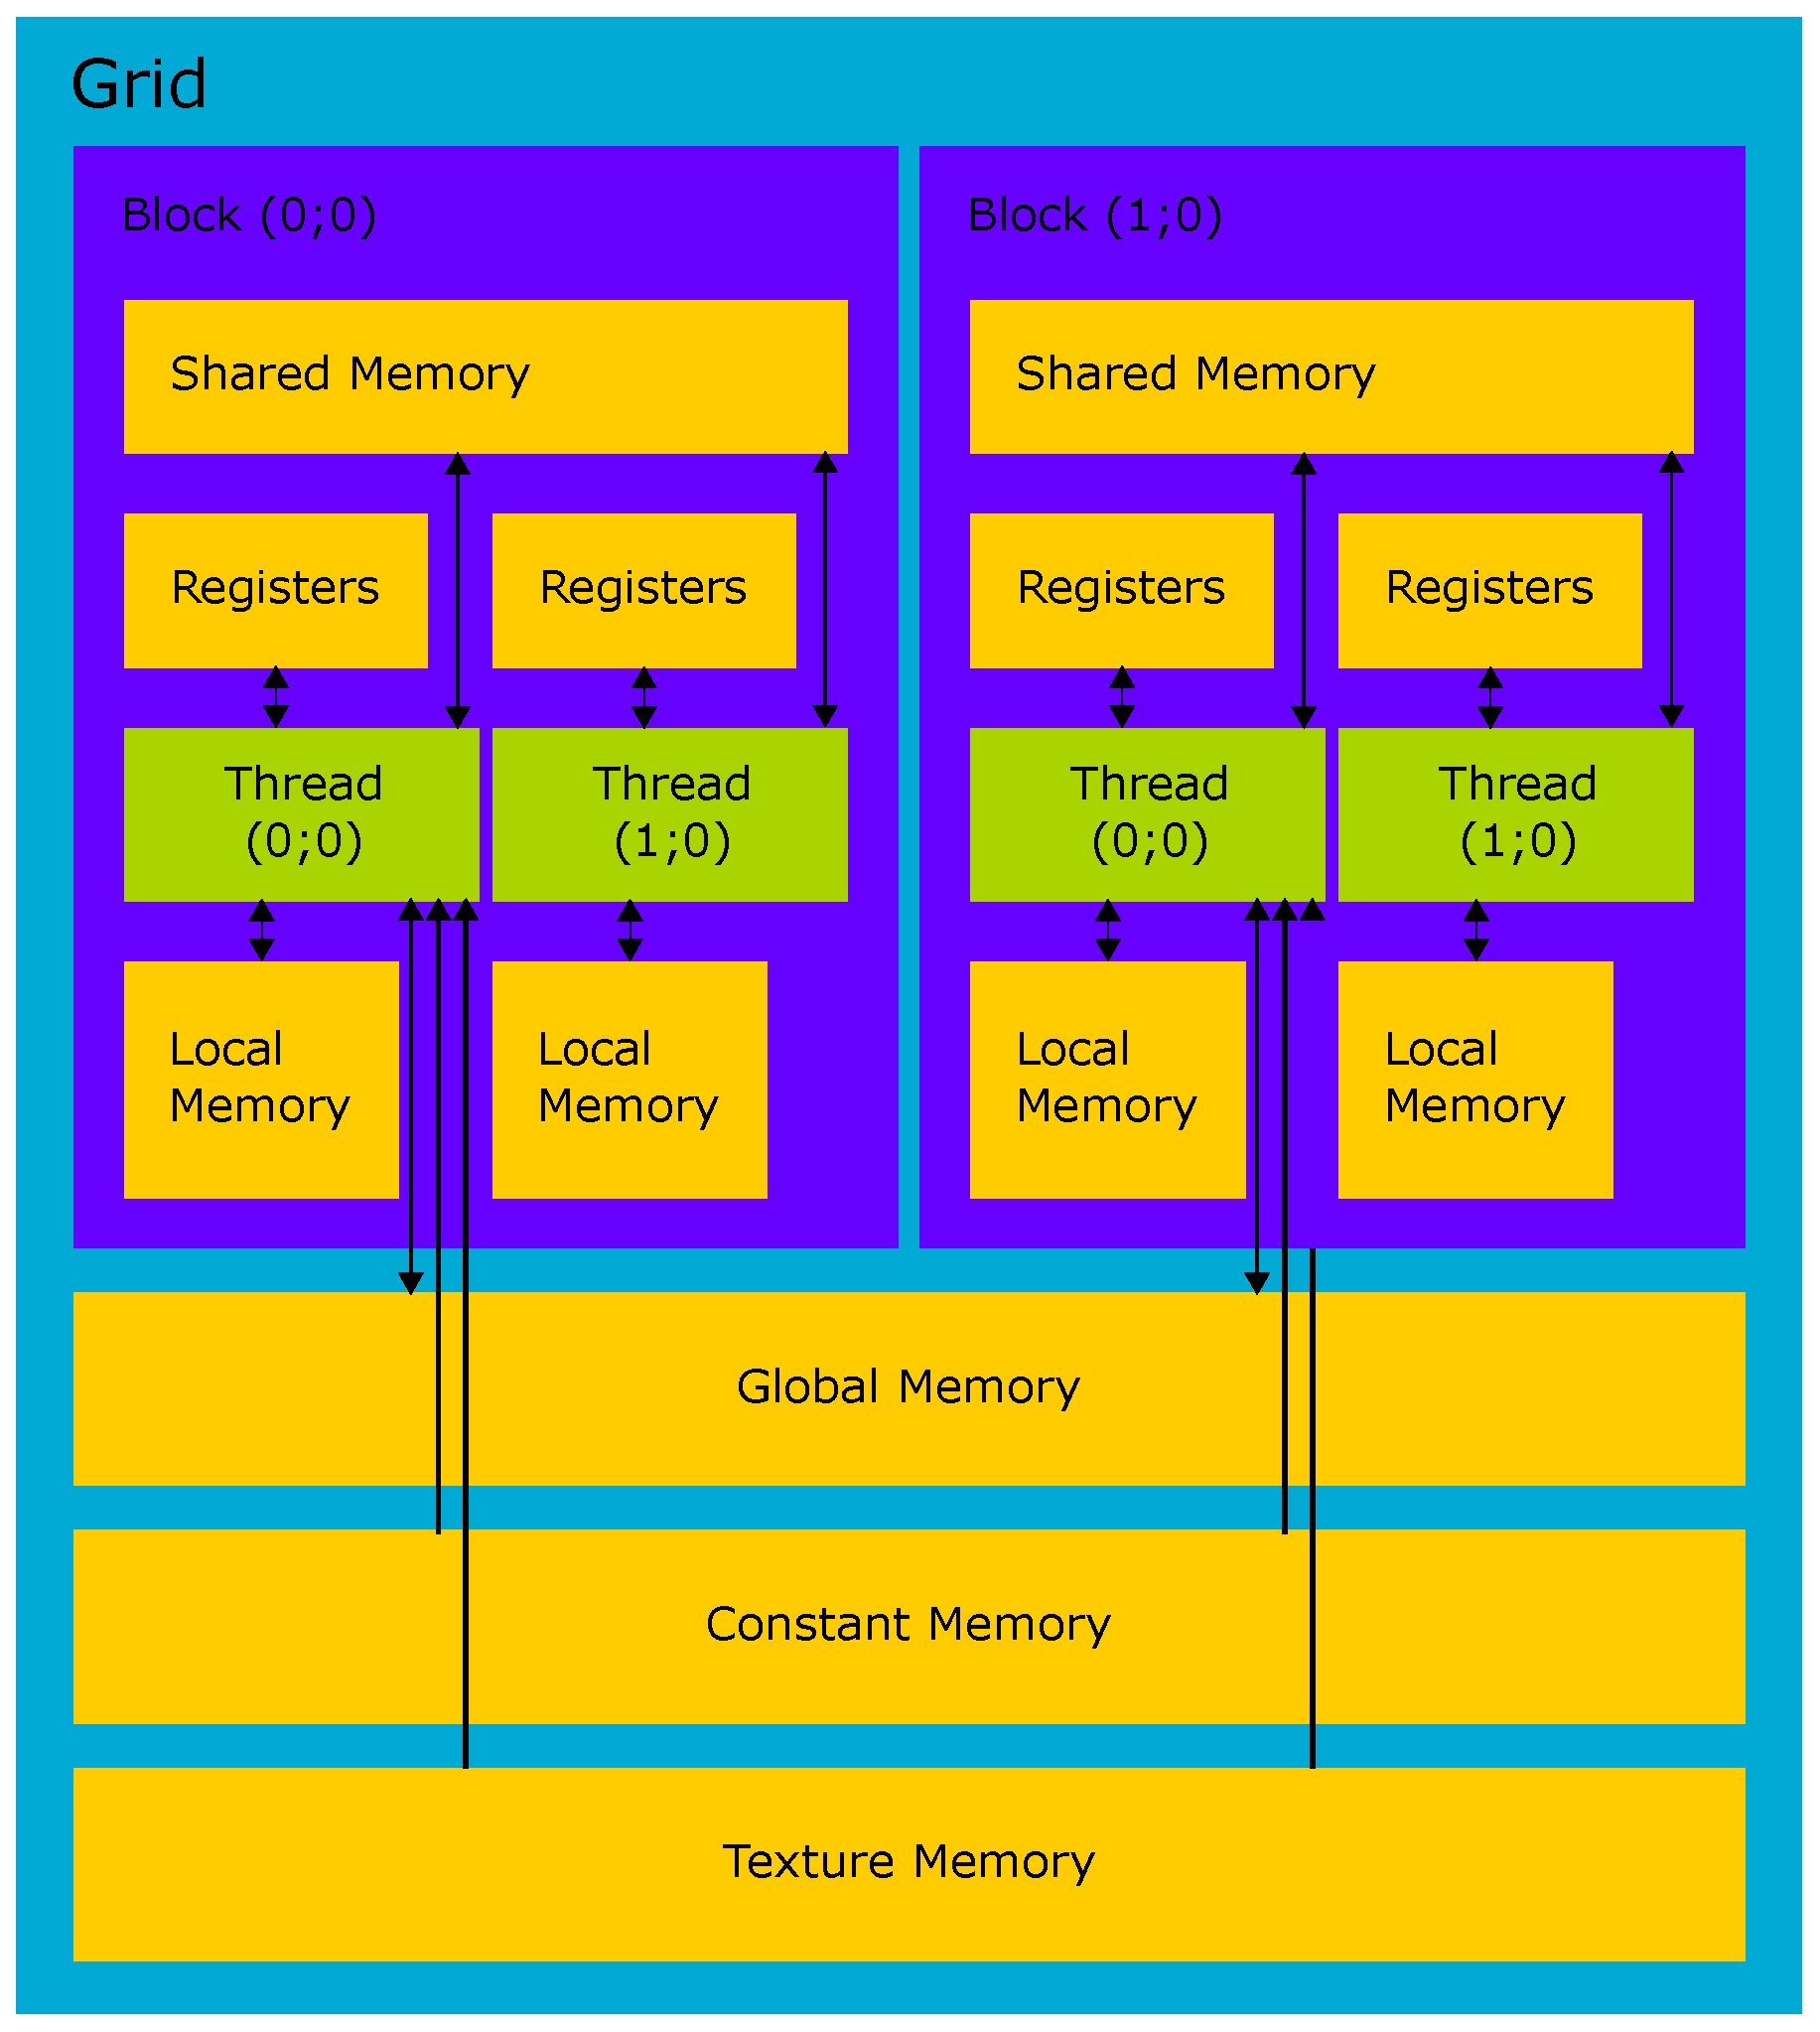
\includegraphics[width=0.6\linewidth]{img/CUDAmemAccess.eps}
  \caption{CUDA Memory access}
  \label{fig:cudamemaccess}
\end{figure}

Data transfer between host and device are much slower than on device memory transfers (16/32 GBps depend on PCI Express version, but could be slowed by host memory), which could make CUDA inefficient for small data and compute inexpensive tasks. Transfer call has great overhead so bulk transfers are preferred over individually transfers. Data are copied from host code to device global memory but host memory could be mapped to the host memory space and than data could be accessed directly from device code (but with same, bad latency). Data transfer could be hidden by overlapping data transfer with computing, because CUDA device is capable of computing and simultaneously perform two asynchronous data transfers.

% is little bit different, because programmer can split execution of instructions into different branches by conditions based on thread identification. In both models